\documentclass{standalone}
%
\usepackage{amsmath}
\usepackage{amsfonts}
\usepackage{amssymb}
\usepackage{amsthm}
\usepackage{mathrsfs}
\usepackage{tikz}
\usetikzlibrary{intersections}
\usetikzlibrary{arrows}
\usetikzlibrary{calc}
\usetikzlibrary{decorations.pathreplacing, decorations.markings}
%\usepackage{amsfonts}
%\usepackage{amsmath}
%\usepackage{amssymb}
%\usepackage{amsthm}
%\usepackage{bbold}
%\usepackage{mathrsfs}
%
\newcommand{\orderO}{\mathcal{O}}
%
\newcommand{\wpar}{w_\parallel}
\newcommand{\wperp}{w_\perp}
%
\newcommand{\kpar}{k_\parallel}
\newcommand{\kperp}{k_\perp}
%
\newcommand{\Lpar}{L_\parallel}
\newcommand{\Lperp}{L_\perp}
%
% - Inhomogeneous RMHD qtys
%
\newcommand{\kpp}{k_p^+}
\newcommand{\kpm}{k_p^-}
\newcommand{\kppm}{k_p^\pm}
\newcommand{\kmp}{k_m^+}
\newcommand{\kmm}{k_m^-}
\newcommand{\kmpm}{k_m^\pm}
\newcommand{\ka}{k_A}
\newcommand{\krho}{k_\rho}
%
% - Special functions
%
\newcommand{\erf}{\mathrm{erf}} % error function
\newcommand{\erfc}{\mathrm{erfc}} % error function
%
% - Proper names
%
\newcommand{\Alfven}{Alfv\'{e}n\ }
%
% - Mathematical Operators
%
\newcommand{\cross}{\boldsymbol{\times}}
\newcommand{\deldot}{\boldsymbol{\nabla\cdot}}
\newcommand{\delperpdot}{\boldsymbol{\nabla_\perp\cdot}}
\newcommand{\delcross}{\boldsymbol{\nabla\times}}
\newcommand{\delperpcross}{\boldsymbol{\nabla_\perp\times}}
\newcommand{\dotdel}{\boldsymbol{\cdot\nabla}}
\newcommand{\dotdelperp}{\boldsymbol{\cdot\nabla_\perp}}
\newcommand{\delperp}{\boldsymbol{\nabla}_\perp}
\newcommand{\delpar}{\boldsymbol{\nabla}_\parallel}
\newcommand{\bfdel}{\boldsymbol{\nabla}}
\newcommand{\pardt}{\partial_t}
\newcommand{\pardx}{\partial_x}
\newcommand{\pardy}{\partial_y}
\newcommand{\pardz}{\partial_z}
\newcommand{\pardzeta}{\partial_\zeta}
\newcommand{\parddt}{\partial_{tt}}
\newcommand{\parddx}{\partial_{xx}}
\newcommand{\parddy}{\partial_{yy}}
\newcommand{\parddz}{\partial_{zz}}
\newcommand{\parddzeta}{\partial_{\zeta\zeta}}
\newcommand{\delsquared}{\nabla^2}
%
% - Bold-Face Vectors
%
\newcommand{\Avec}{\mathbf{A}}
\newcommand{\Bvec}{\mathbf{B}}
\newcommand{\Cvec}{\mathbf{C}}
\newcommand{\Dvec}{\mathbf{D}}
\newcommand{\Evec}{\mathbf{E}}
\newcommand{\Fvec}{\mathbf{F}}
\newcommand{\Gvec}{\mathbf{G}}
\newcommand{\Hvec}{\mathbf{H}}
\newcommand{\Ivec}{\mathbf{I}}
\newcommand{\Jvec}{\mathbf{J}}
\newcommand{\Kvec}{\mathbf{K}}
\newcommand{\Lvec}{\mathbf{L}}
\newcommand{\Mvec}{\mathbf{M}}
\newcommand{\Nvec}{\mathbf{N}}
\newcommand{\Ovec}{\mathbf{O}}
\newcommand{\Pvec}{\mathbf{P}}
\newcommand{\Qvec}{\mathbf{Q}}
\newcommand{\Rvec}{\mathbf{R}}
\newcommand{\Svec}{\mathbf{S}}
\newcommand{\Tvec}{\mathbf{T}}
\newcommand{\Uvec}{\mathbf{U}}
\newcommand{\Vvec}{\mathbf{V}}
\newcommand{\Wvec}{\mathbf{W}}
\newcommand{\Xvec}{\mathbf{X}}
\newcommand{\Yvec}{\mathbf{Y}}
\newcommand{\Zvec}{\mathbf{Z}}
\newcommand{\avec}{\mathbf{a}}
\newcommand{\bvec}{\mathbf{b}}
\newcommand{\cvec}{\mathbf{c}}
\newcommand{\dvec}{\mathbf{d}}
\newcommand{\evec}{\mathbf{e}}
\newcommand{\fvec}{\mathbf{f}}
\newcommand{\gvec}{\mathbf{g}}
\newcommand{\hvec}{\mathbf{h}}
\newcommand{\ivec}{\mathbf{i}}
\newcommand{\jvec}{\mathbf{j}}
\newcommand{\kvec}{\mathbf{k}}
\newcommand{\lvec}{\mathbf{l}}
\newcommand{\mvec}{\mathbf{m}}
\newcommand{\nvec}{\mathbf{n}}
\newcommand{\ovec}{\mathbf{o}}
\newcommand{\pvec}{\mathbf{p}}
\newcommand{\qvec}{\mathbf{q}}
\newcommand{\rvec}{\mathbf{r}}
\newcommand{\svec}{\mathbf{s}}
\newcommand{\tvec}{\mathbf{t}}
\newcommand{\uvec}{\mathbf{u}}
\newcommand{\vvec}{\mathbf{v}}
\newcommand{\wvec}{\mathbf{w}}
\newcommand{\xvec}{\mathbf{x}}
\newcommand{\yvec}{\mathbf{y}}
\newcommand{\zvec}{\mathbf{z}}

% - Elsasser Variable related
%
\newcommand{\elsasser}{Els\"{a}sser}
%
\newcommand{\elsaspm}{\avec^{\pm}}
\newcommand{\elsasmp}{\avec^{\mp}}
\newcommand{\elsasp}{\avec^{+}}
\newcommand{\elsasm}{\avec^{-}}
%
\newcommand{\elsasxpm}{a_x^{\pm}}
\newcommand{\elsasypm}{a_y^{\pm}}
\newcommand{\elsasxmp}{a_x^{\mp}}
\newcommand{\elsasymp}{a_y^{\mp}}
%
\newcommand{\elsasOmpm}{\Omega^{\pm}}
\newcommand{\elsasOmmp}{\Omega^{\mp}}
\newcommand{\elsasOmp}{\Omega^{+}}
\newcommand{\elsasOmm}{\Omega^{-}}
%
\newcommand{\elsasompm}{\omega^{\pm}}
\newcommand{\elsasommp}{\omega^{\mp}}
\newcommand{\elsasomp}{\omega^{+}}
\newcommand{\elsasomm}{\omega^{-}}
%
\newcommand{\elsasphipm}{\phi^{\pm}}
\newcommand{\elsasphimp}{\phi^{\mp}}
\newcommand{\elsasphip}{\phi^{+}}
\newcommand{\elsasphim}{\phi^{-}}
%
\newcommand{\elsaspsipm}{\psi^{\pm}}
\newcommand{\elsaspsimp}{\psi^{\mp}}
\newcommand{\elsaspsip}{\psi^{+}}
\newcommand{\elsaspsim}{\psi^{-}}
%
% - Common functional dependencies and intregration elements

\newcommand{\ofrvecvvecnt}{(\rvec,\vvec,t)}
\newcommand{\ofrvecvvec}{(\rvec,\vvec)}
\newcommand{\ofrvecnt}{(\rvec,t)}
\newcommand{\ofrvec}{(\rvec)}
\newcommand{\ofxnv}{(x,v)}
\newcommand{\ofznv}{(z,v)}
\newcommand{\ofznvz}{(z,v_z}
\newcommand{\ofrhoznvz}{(\rho,z,v_z)}
\newcommand{\ofrhonz}{(\rho,z)}
\newcommand{\dcubedv}{\,d^3v}

% - Kinetic Energy Quantities

\newcommand{\kepar}{W_\parallel}
\newcommand{\keperp}{W_\perp}

% - Electric / Magnetic Field Quantities

    % --> magnitudes 
    \newcommand{\magEperp}{E_\perp}
    \newcommand{\magEpar}{E_\parallel}
    \newcommand{\magBperp}{B_\perp}
    \newcommand{\magBpar}{B_\parallel}

    % --> field vectors 
    \newcommand{\Eperp}{\Evec_\perp}
    \newcommand{\Epar}{\Evec_\parallel}
    \newcommand{\Bperp}{\Bvec_\perp}
    \newcommand{\Bpar}{\Bvec_\parallel}

    % --> other field quantities 
    \newcommand{\magBtor}{B_T}                 % Toroidal field strength
    \newcommand{\jpar}{\jvec_\parallel}        % parallel current density
    \newcommand{\jperp}{\jvec_\perp}           % perpendicular current density

    %--> unit vectors
    \newcommand{\bhat}{\hat\bvec}
    \newcommand{\bperphat}{\hat\bvec_\perp}
    \newcommand{\bparhat}{\hat\bvec_\parallel}

% - Discplacements

    \newcommand{\xperp}{\xvec_\perp}
    \newcommand{\xpar}{\xvec_\parallel}

% - Speeds, Velocities, and Vorticities

    \newcommand{\vorticity}{\mathbf{\Omega}}
    \newcommand{\magvorticity}{\Omega}

    % - single fluid 

    % --> magnitudes 

    \newcommand{\talfven}{\tau_{\mathrm{A}}}    % Alfven time
    \newcommand{\magvperp}{v_\perp}             % perpendicular velocity magnitude
    \newcommand{\magvpar}{v_\parallel}          % parallel velocity magnitude
    \newcommand{\magvalfven}{v_{\mathrm{A}}}    % Alfven speed
    \newcommand{\magvthermal}{v_{t}}            % thermal speed

    % --> vectors 
    \newcommand{\vperp}{\vvec_\perp}            % perpendicular velocity
    \newcommand{\vpar}{\vvec_\parallel}         % parallel velocity
    \newcommand{\valfven}{\vvec_{A}}            % Alfven velocity

    % - two fluid 

    % --> magnitudes 

    \newcommand{\magve}{v_e}                    % magnitude electron velocity magnitude
    \newcommand{\magvi}{v_i}                    % magnitude ion velocity magnitude
    \newcommand{\magvs}{v_s}                    % magnitude species velocity magnitude

    \newcommand{\magveperp}{v_{e,\perp}}        % magnitude perpendicular electron perpendicular velocity magnitude
    \newcommand{\magvepar}{v_{e,\parallel}}     % magnitude parallel electron parallel velocity magnitude

    \newcommand{\magviperp}{v_{i,\perp}}        % magnitude ion perpendicular velocity magnitude
    \newcommand{\magvipar}{v_{i,\parallel}}     % magnitude ion parallel velocity magnitude

    \newcommand{\magvsperp}{v_{s,\perp}}        % magnitude species perpendicular velocity magnitude
    \newcommand{\magvspar}{v_{s,\parallel}}     % magnitude species parallel velocity magnitude

    \newcommand{\magvethermal}{v_{e,t}}         % magnitude electron thermal velocity
    \newcommand{\magvithermal}{v_{i,t}}         % magnitude ion thermal velocity
    \newcommand{\magvsthermal}{v_{s,t}}         % magnitude species thermal velocity

    % --> vectors 

    \newcommand{\ve}{\vvec_e}                   % electron velocity
    \newcommand{\vi}{\vvec_i}                   % ion velocity
    \newcommand{\vs}{\vvec_s}                   % species velocity

    \newcommand{\veperp}{\vvec_{e,\perp}}       % perpendicular electron velocity electron perpendicular velocity
    \newcommand{\vepar}{\vvec_{e,\parallel}}    % parallel electron velocity electron parallel velocity

    \newcommand{\viperp}{\vvec_{i,\perp}}       % perpendicular ion velocity ion perpendicular velocity
    \newcommand{\vipar}{\vvec_{i,\parallel}}    % parallel ion velocity ion parallel velocity

    \newcommand{\vsperp}{\vvec_{s,\perp}}       % species perpendicular velocity
    \newcommand{\vspar}{\vvec_{s,\parallel}}    % species parallel velocity

% - Geometric Quantities

    % - unit vectors

    \newcommand{\xhat}{\hat\xvec}
    \newcommand{\yhat}{\hat\yvec}
    \newcommand{\zhat}{\hat\zvec}

    \newcommand{\rhohat}{\boldsymbol{\hat\rho}}
    \newcommand{\phihat}{\boldsymbol{\hat\phi}}

    \newcommand{\eperphat}{\hat\evec_\perp}
    \newcommand{\eparhat}{\hat\evec_\parallel}

\newcommand{\Radcurv}{\Rvec_c} % - radius of curvature

\newcommand{\Radcurvmag}{R_c}  % - magnitude radius of curvature

% Thermodynamic Quantities

   %--> number/particle densities
   \newcommand{\nedens}{n_e}  % - electron density
   \newcommand{\nidens}{n_i}  % - ion density
   \newcommand{\npdens}{n_p}  % - proton density
   \newcommand{\nsdens}{n_s}  % - species density
   \newcommand{\nndens}{n_0}  % - neutral density
   %--> temperatures (isotropic)
   \newcommand{\etemp}{T_e}   % - electron temperature
   \newcommand{\ptemp}{T_p}   % - proton temperature
   \newcommand{\itemp}{T_i}   % - ion temperature
   \newcommand{\stemp}{T_s}   % - species temperature
   \newcommand{\gtemp}{T}     % - generic temperature
   %--> temperatures (anisotropic)
   \newcommand{\etempperp}{T_e^\perp} % - perpendicular electron temperature
   \newcommand{\ptempperp}{T_p^\perp}   % - perpendicular proton temperature
   \newcommand{\itempperp}{T_i^\perp}   % - perpendicular ion temperature
   \newcommand{\stempperp}{T_s^\perp}   % - perpendicular species temperature

   \newcommand{\etemppar}{T_e^\parallel}   % - parallel electron temperature
   \newcommand{\ptemppar}{T_p^\parallel}   % - parallel proton temperature
   \newcommand{\itemppar}{T_i^\parallel}   % - parallel ion temperature
   \newcommand{\stemppar}{T_s^\parallel}   % - parallel species temperature

   %-- pressures (species)

   \newcommand{\epres}{P_e} % electron pressure
   \newcommand{\ipres}{P_i} % ion pressure
   \newcommand{\spres}{P_s} % species pressure

   %-- vectors

   \newcommand{\eifric}{\mathboldsans{\Gamma}} % electron-ion friction
   \newcommand{\qeflux}{\qvec_e}               % electron heat flux
   \newcommand{\qiflux}{\qvec_i}               % ion heat flux
   \newcommand{\qsflux}{\qvec_s}               % species heat flux

   %-- tensors
   
   \newcommand{\estresst}{\mathboldsans{\Pi}_e}      % electron stress tensor
   \newcommand{\istresst}{\mathboldsans{\Pi}_i}      % ion stress tensor
   \newcommand{\eistresst}{\mathboldsans{\Pi}_{e,i}} % electron or ion stress tensor
   \newcommand{\sstresst}{\mathboldsans{\Pi}_{s}}    % species stress tensor
   \newcommand{\stresst}{\mathboldsans{\Pi}}         % generic stress tensor

   \newcommand{\stresscomp}{\mathsf{\Pi}}            % generic stress tensor component root


   \newcommand{\rostrain}{\mathboldsans{W}}          % Rate-of-strain tensor
   \newcommand{\rostraincomp}{\mathsf{W}}            % Rate-of-strain tensor component root

% Units

\newcommand{\percc}{\mathrm{cm}^{-3}}
\newcommand{\kelvin}{\mathrm{K}}
\newcommand{\radspersec}{\mathrm{rad/s}}
\newcommand{\hertz}{\mathrm{Hz}}
\newcommand{\percm}{\mathrm{m}^{-3}}
\newcommand{\persec}{\mathrm{sec}^{-1}}
\newcommand{\coulomb}{\mathrm{C}}
\newcommand{\eV}{\mathrm{eV}}

% physical constants

\newcommand{\kboltz}{k_{\mathrm{B}}}
\newcommand{\epszero}{\epsilon_0}
\newcommand{\muzero}{\mu_0}

% plasma parameters 

\newcommand{\debyelength}{\lambda_{\mathrm{D}}} % debye length
\newcommand{\edebyelength}{\lambda_{e}}         % electron debye length

\newcommand{\elmass}{m_e}          % electron mass
\newcommand{\prmass}{m_p}          % proton mass
\newcommand{\iomass}{m_i}          % ion mass
\newcommand{\spmass}{m_s}          % species mass

\newcommand{\elplfr}{\omega_{p,e}} % electron plasma frequency larmor Larmor cyclotron
\newcommand{\prplfr}{\omega_{p,p}} % proton plasma frequency
\newcommand{\ioplfr}{\omega_{p,i}} % ion plasma frequency
\newcommand{\spplfr}{\omega_{p,s}} % species plasma frequency

\newcommand{\elgyrorad}{\rho_e}    % electron gyroradius
\newcommand{\prgyrorad}{\rho_p}    % proton gyroradius
\newcommand{\iogyrorad}{\rho_i}    % ion gyroradius
\newcommand{\spgyrorad}{\rho_s}    % species gyroradius

\newcommand{\elgyrofreq}{\Omega_e} % electron gyrofrequency
\newcommand{\prgyrofreq}{\Omega_p} % proton gyrofrequency
\newcommand{\iogyrofreq}{\Omega_i} % ion gyrofrequency
\newcommand{\spgyrofreq}{\Omega_s} % species gyrofrequency
\newcommand{\gegyrofreq}{\Omega}   % generic gyrofrequency

\newcommand{\etcol}{\tau_e}        % electron collision time 
\newcommand{\itcol}{\tau_i}        % ion collision time 
\newcommand{\stcol}{\tau_s}        % species collision time 
\newcommand{\tcol}{\tau}           % generic collision time 

\newcommand{\condpar}{\sigma_\parallel} % parallel electrical conductivity
\newcommand{\condperp}{\sigma_\perp}    % perpendicular electrical conductivity
\newcommand{\condnom}{\sigma_0}         % nominal conductivity constant (see Breginskii 65 where it's called sigma_1)

\newcommand{\visc}{\nu}                 % some changeable greek letter for representing viscosity coefficients

\newcommand{\parvisc}{\visc_\parallel}  % parallel      viscosity as understood in the manner of Biskamp's discussion
\newcommand{\perpvisc}{\visc_\perp}     % perpendicular viscosity as understood in the manner of Biskamp's discussion
\newcommand{\gyrovisc}{\visc_g}         % ``non-dissipative'' gyroviscosity as understood in the manner of Biskamp's discussion

\newcommand{\viscconstpar}{c_\parallel}  % numerical constant for parallel viscosity
\newcommand{\viscconstperp}{c_\perp}     % numerical constant for perpendicular viscosity
\newcommand{\viscconstgyro}{c_g}         % numerical constant for gyro viscosity

% Operators


% miscellaneous

\newcommand{\ecrossb}{\Evec\times\Bvec}



\newcommand{\hfield}{\mathscr{H}}
%
\tikzset{
	on each segment/.style={
		decorate,
		decoration={
			show path construction,
			moveto code={},
			lineto code={
				\path [#1]
				(\tikzinputsegmentfirst) -- (\tikzinputsegmentlast);
			},
			curveto code={
				\path [#1] (\tikzinputsegmentfirst)
				..controls
				(\tikzinputsegmentsupporta) and (\tikzinputsegmentsupportb)
				..
				(\tikzinputsegmentlast);
			},
			closepath code={
				\path [#1]
				(\tikzinputsegmentfirst) -- (\tikzinputsegmentlast);
			},
		},
	},
	mid arrow/.style={postaction={decorate,decoration={
		markings,
		mark= at position .5 with {\arrow[#1]{stealth}}
	}}},
	reverse mid arrow/.style={postaction={decorate,decoration={
		markings,
		mark= at position .5 with {\arrowreversed[#1]{stealth}}
	}}},
}
%
\begin{document}
 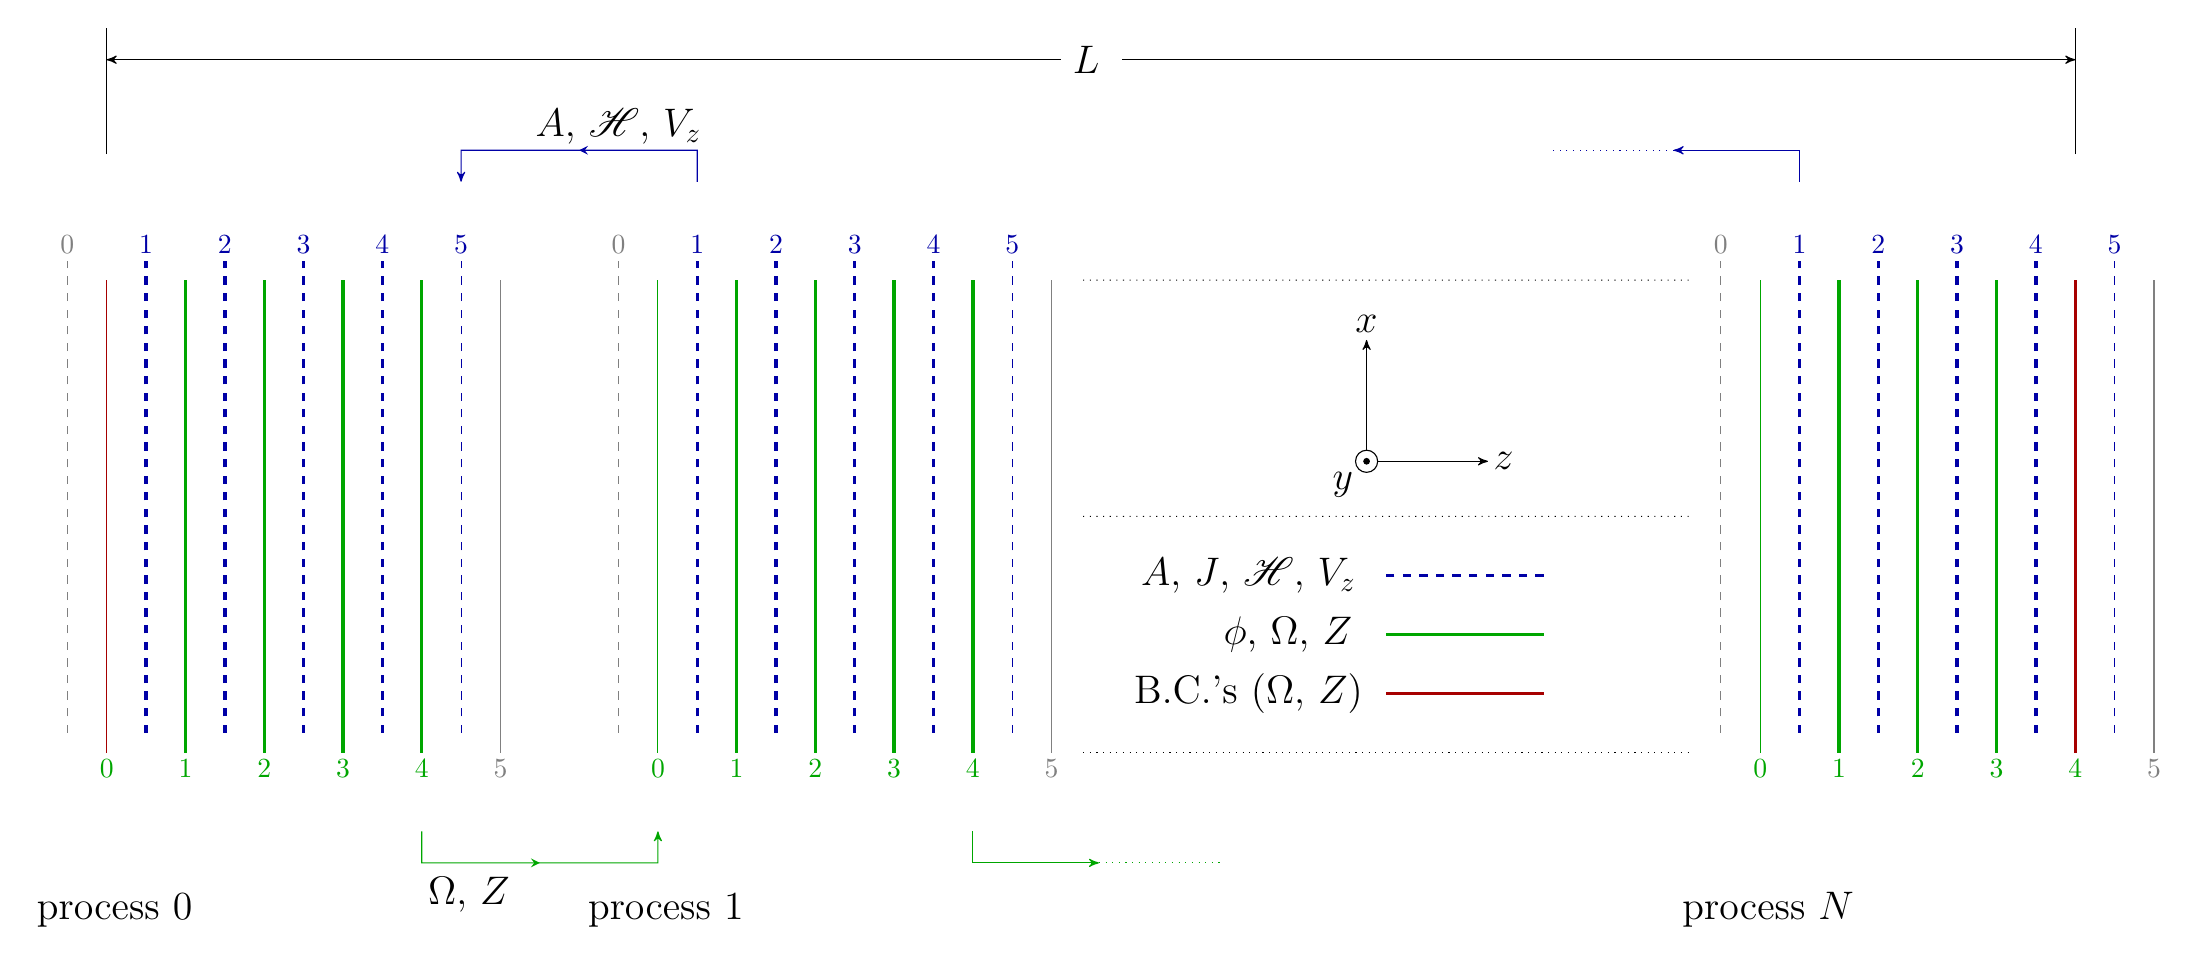
\begin{tikzpicture}[scale=2.0, >=stealth']
%
% ~~~~~~~~~~~~~~~~~~~~~~~~~~~~~~~~~~~~~~~~~~~~~~~~~~~~~~~~~~~~~~~~~~~~~~~~~~~~~~~~~~~~~~~~~~~~~~~~~~~~~~~~~~~~~~~~~~~~~~~~~~~~~~~~ %
% ~ coordinates ~~~~~~~~~~~~~~~~~~~~~~~~~~~~~~~~~~~~~~~~~~~~~~~~~~~~~~~~~~~~~~~~~~~~~~~~~~~~~~~~~~~~~~~~~~~~~~~~~~~~~~~~~~~~~~~~~~ %
% ~~~~~~~~~~~~~~~~~~~~~~~~~~~~~~~~~~~~~~~~~~~~~~~~~~~~~~~~~~~~~~~~~~~~~~~~~~~~~~~~~~~~~~~~~~~~~~~~~~~~~~~~~~~~~~~~~~~~~~~~~~~~~~~~ %
%
% ~ for rank 0 Grid A (specification of A, J) ~ %
%
\coordinate  (g0a0l) at (0.000cm,0.125cm);
\coordinate  (g0a0h) at ($(g0a0l) + (0.0cm, 3.0cm)$);
%
\coordinate  (g0a1l) at ($(g0a0l) + (0.5cm, 0.0cm)$);
\coordinate  (g0a1h) at ($(g0a1l) + (0.0cm, 3.0cm)$);
%
\coordinate  (g0a2l) at ($(g0a1l) + (0.5cm, 0.0cm)$);
\coordinate  (g0a2h) at ($(g0a2l) + (0.0cm, 3.0cm)$);
%
\coordinate  (g0a3l) at ($(g0a2l) + (0.5cm, 0.0cm)$);
\coordinate  (g0a3h) at ($(g0a3l) + (0.0cm, 3.0cm)$);
%
\coordinate  (g0a4l) at ($(g0a3l) + (0.5cm, 0.0cm)$);
\coordinate  (g0a4h) at ($(g0a4l) + (0.0cm, 3.0cm)$);
%
\coordinate  (g0a5l) at ($(g0a4l) + (0.5cm, 0.0cm)$);
\coordinate  (g0a5h) at ($(g0a5l) + (0.0cm, 3.0cm)$);
%
% ~ for rank 0 Grid B (specification of phi, Omega) ~ %
%
\coordinate  (g0b0l) at (0.250cm, 0.000cm);
\coordinate  (g0b0h) at ($(g0b0l) + (0.0cm, 3.0cm)$);
%
\coordinate  (g0b1l) at ($(g0b0l) + (0.5cm, 0.0cm)$);
\coordinate  (g0b1h) at ($(g0b1l) + (0.0cm, 3.0cm)$);
%
\coordinate  (g0b2l) at ($(g0b1l) + (0.5cm, 0.0cm)$);
\coordinate  (g0b2h) at ($(g0b2l) + (0.0cm, 3.0cm)$);
%
\coordinate  (g0b3l) at ($(g0b2l) + (0.5cm, 0.0cm)$);
\coordinate  (g0b3h) at ($(g0b3l) + (0.0cm, 3.0cm)$);
%
\coordinate  (g0b4l) at ($(g0b3l) + (0.5cm, 0.0cm)$);
\coordinate  (g0b4h) at ($(g0b4l) + (0.0cm, 3.0cm)$);
%
\coordinate  (g0b5l) at ($(g0b4l) + (0.5cm, 0.0cm)$);
\coordinate  (g0b5h) at ($(g0b5l) + (0.0cm, 3.0cm)$);
%
% ~ for rank 1 Grid A (specification of A, J) ~ %
%
\coordinate  (g1a0l) at (3.500cm,0.125cm);
\coordinate  (g1a0h) at ($(g1a0l) + (0.0cm, 3.0cm)$);
%
\coordinate  (g1a1l) at ($(g1a0l) + (0.5cm, 0.0cm)$);
\coordinate  (g1a1h) at ($(g1a1l) + (0.0cm, 3.0cm)$);
%
\coordinate  (g1a2l) at ($(g1a1l) + (0.5cm, 0.0cm)$);
\coordinate  (g1a2h) at ($(g1a2l) + (0.0cm, 3.0cm)$);
%
\coordinate  (g1a3l) at ($(g1a2l) + (0.5cm, 0.0cm)$);
\coordinate  (g1a3h) at ($(g1a3l) + (0.0cm, 3.0cm)$);
%
\coordinate  (g1a4l) at ($(g1a3l) + (0.5cm, 0.0cm)$);
\coordinate  (g1a4h) at ($(g1a4l) + (0.0cm, 3.0cm)$);
%
\coordinate  (g1a5l) at ($(g1a4l) + (0.5cm, 0.0cm)$);
\coordinate  (g1a5h) at ($(g1a5l) + (0.0cm, 3.0cm)$);
%
% ~ for rank 1 Grid B (specification of phi, Omega) ~ %
%
\coordinate  (g1b0l) at (3.750cm, 0.000cm);
\coordinate  (g1b0h) at ($(g1b0l) + (0.0cm, 3.0cm)$);
%
\coordinate  (g1b1l) at ($(g1b0l) + (0.5cm, 0.0cm)$);
\coordinate  (g1b1h) at ($(g1b1l) + (0.0cm, 3.0cm)$);
%
\coordinate  (g1b2l) at ($(g1b1l) + (0.5cm, 0.0cm)$);
\coordinate  (g1b2h) at ($(g1b2l) + (0.0cm, 3.0cm)$);
%
\coordinate  (g1b3l) at ($(g1b2l) + (0.5cm, 0.0cm)$);
\coordinate  (g1b3h) at ($(g1b3l) + (0.0cm, 3.0cm)$);
%
\coordinate  (g1b4l) at ($(g1b3l) + (0.5cm, 0.0cm)$);
\coordinate  (g1b4h) at ($(g1b4l) + (0.0cm, 3.0cm)$);
%
\coordinate  (g1b5l) at ($(g1b4l) + (0.5cm, 0.0cm)$);
\coordinate  (g1b5h) at ($(g1b5l) + (0.0cm, 3.0cm)$);
%
% ~ for rank N Grid A (specification of A, J) ~ %
%
\coordinate  (gna0l) at (10.500cm,0.125cm);
\coordinate  (gna0h) at ($(gna0l) + (0.0cm, 3.0cm)$);
%
\coordinate  (gna1l) at ($(gna0l) + (0.5cm, 0.0cm)$);
\coordinate  (gna1h) at ($(gna1l) + (0.0cm, 3.0cm)$);
%
\coordinate  (gna2l) at ($(gna1l) + (0.5cm, 0.0cm)$);
\coordinate  (gna2h) at ($(gna2l) + (0.0cm, 3.0cm)$);
%
\coordinate  (gna3l) at ($(gna2l) + (0.5cm, 0.0cm)$);
\coordinate  (gna3h) at ($(gna3l) + (0.0cm, 3.0cm)$);
%
\coordinate  (gna4l) at ($(gna3l) + (0.5cm, 0.0cm)$);
\coordinate  (gna4h) at ($(gna4l) + (0.0cm, 3.0cm)$);
%
\coordinate  (gna5l) at ($(gna4l) + (0.5cm, 0.0cm)$);
\coordinate  (gna5h) at ($(gna5l) + (0.0cm, 3.0cm)$);
%
% ~ for rank N Grid B (specification of phi, Omega) ~ %
%
\coordinate  (gnb0l) at (10.750cm, 0.000cm);
\coordinate  (gnb0h) at ($(gnb0l) + (0.0cm, 3.0cm)$);
%
\coordinate  (gnb1l) at ($(gnb0l) + (0.5cm, 0.0cm)$);
\coordinate  (gnb1h) at ($(gnb1l) + (0.0cm, 3.0cm)$);
%
\coordinate  (gnb2l) at ($(gnb1l) + (0.5cm, 0.0cm)$);
\coordinate  (gnb2h) at ($(gnb2l) + (0.0cm, 3.0cm)$);
%
\coordinate  (gnb3l) at ($(gnb2l) + (0.5cm, 0.0cm)$);
\coordinate  (gnb3h) at ($(gnb3l) + (0.0cm, 3.0cm)$);
%
\coordinate  (gnb4l) at ($(gnb3l) + (0.5cm, 0.0cm)$);
\coordinate  (gnb4h) at ($(gnb4l) + (0.0cm, 3.0cm)$);
%
\coordinate  (gnb5l) at ($(gnb4l) + (0.5cm, 0.0cm)$);
\coordinate  (gnb5h) at ($(gnb5l) + (0.0cm, 3.0cm)$);
%
% ~ for passing atop down to previous rank           ~ %
%
\coordinate  (pas)   at ($(g0a5h) + (0.0cm,0.5cm)$);
\coordinate  (pau)   at ($(pas)   + (0.0cm,0.2cm)$);
\coordinate  (par)   at ($(g1a1h) + (0.0cm,0.7cm)$);
\coordinate  (pad)   at ($(par)   - (0.0cm,0.2cm)$);
%
\coordinate  (par1)   at ($(gna1h) + (0.0cm,0.5cm)$);
\coordinate  (pau1)   at ($(par1)  + (0.0cm,0.2cm)$);
\coordinate  (pam1)   at ($(pau1)  - (0.8cm,0.0cm)$);
\coordinate  (pas1)   at ($(pam1)  - (0.8cm,0.0cm)$);
%
% ~ for passing pbot up to next rank                ~ %
%
\coordinate  (pps)   at ($(g0b4l) - (0.0cm,0.5cm)$);
\coordinate  (ppu)   at ($(pps)   - (0.0cm,0.2cm)$);
\coordinate  (ppr)   at ($(g1b0l) - (0.0cm,0.7cm)$);
\coordinate  (ppd)   at ($(ppr)   + (0.0cm,0.2cm)$);
%
\coordinate  (pps1)   at ($(g1b4l) - (0.0cm,0.5cm)$);
\coordinate  (ppu1)   at ($(pps1)  - (0.0cm,0.2cm)$);
\coordinate  (ppm1)   at ($(ppu1)  + (0.8cm,0.0cm)$);
\coordinate  (ppr1)   at ($(ppm1)  + (0.8cm,0.0cm)$);
%
% ~ for labeling rank of stack                      ~ %
%
\coordinate (s0lab)  at (0.0cm,-1.0cm);
\coordinate (s1lab)  at ($(g1b0l) + (-0.25cm,-1.0cm)$);
\coordinate (snlab)  at ($(gnb0l) + (-0.25cm,-1.0cm)$);
%
% ~ for specifying column length                    ~ %
%
\coordinate (hshll)  at ($(g0b0h) + (0.0cm, 0.8cm)$);
\coordinate (hshhl)  at ($(hshll) + (0.0cm, 0.8cm)$);
%
\coordinate (hshlr)  at ($(gnb4h) + (0.0cm, 0.8cm)$);
\coordinate (hshhr)  at ($(hshlr) + (0.0cm, 0.8cm)$);
%
\coordinate (lwarl)  at ($(hshll) + (0.0cm, 0.6cm)$); 
\coordinate (rwarr)  at ($(hshlr) + (0.0cm, 0.6cm)$); 
%
% ~ for showing Cartesian axes                      ~ %
%
\coordinate (orig)   at ($(g1b5l) + (2.0cm, 1.85cm)$);

% ~ for indicating field specifications             ~ %
%
\coordinate (gridal) at ($(g1b5l)    + (2.125cm, 1.125cm)$);
\coordinate (gridar) at ($(gridal)   + (1.0cm, 0.000cm)$);
%
\coordinate (gridbl) at ($(g1b5l)    + (2.125cm, 0.75cm)$);
\coordinate (gridbr) at ($(gridbl)   + (1.0cm, 0.00cm)$);
%
\coordinate (gridbcl) at ($(g1b5l)   + (2.125cm, 0.375cm)$);
\coordinate (gridbcr) at ($(gridbcl) + (1.0cm, 0.00cm)$);

% ~~~~~~~~~~~~~~~~~~~~~~~~~~~~~~~~~~~~~~~~~~~~~~~~~~~~~~~~~~~~~~~~~~~~~~~~~~~~~~~~~~~~~~~~~~~~~~~~~~~~~~~~~~~~~~~~~~~~~~~~~~~~~~~~ %
% ~ grid layers ~~~~~~~~~~~~~~~~~~~~~~~~~~~~~~~~~~~~~~~~~~~~~~~~~~~~~~~~~~~~~~~~~~~~~~~~~~~~~~~~~~~~~~~~~~~~~~~~~~~~~~~~~~~~~~~~~~ %
% ~~~~~~~~~~~~~~~~~~~~~~~~~~~~~~~~~~~~~~~~~~~~~~~~~~~~~~~~~~~~~~~~~~~~~~~~~~~~~~~~~~~~~~~~~~~~~~~~~~~~~~~~~~~~~~~~~~~~~~~~~~~~~~~~ %
%
% ~ for rank 0 Grid A (specification of A, J) ~ %
%
\draw[         gray, dashed] (g0a0l) -- (g0a0h) node [ yshift = 0.2cm ] { $0$ };
\draw[very thick,blue!65!black, dashed] (g0a1l) -- (g0a1h) node [ yshift = 0.2cm ] { $1$ };
\draw[very thick,blue!65!black, dashed] (g0a2l) -- (g0a2h) node [ yshift = 0.2cm ] { $2$ };
\draw[very thick,blue!65!black, dashed] (g0a3l) -- (g0a3h) node [ yshift = 0.2cm ] { $3$ };
\draw[very thick,blue!65!black, dashed] (g0a4l) -- (g0a4h) node [ yshift = 0.2cm ] { $4$ };
\draw[blue!65!black, dashed] (g0a5l) -- (g0a5h) node [ yshift = 0.2cm ] { $5$ };
%
% ~ for rank 0 Grid B (specification of phi, Omega) ~ %
%
\draw[red!65!black] (g0b0h) -- (g0b0l) node [ yshift = -0.2cm ,green!65!black] { $0$ };
\draw[very thick,green!65!black] (g0b1h) -- (g0b1l) node [ yshift = -0.2cm ]   { $1$ };
\draw[very thick,green!65!black] (g0b2h) -- (g0b2l) node [ yshift = -0.2cm ]   { $2$ };
\draw[very thick,green!65!black] (g0b3h) -- (g0b3l) node [ yshift = -0.2cm ]   { $3$ };
\draw[very thick,green!65!black] (g0b4h) -- (g0b4l) node [ yshift = -0.2cm ]   { $4$ };
\draw[gray] (g0b5h) -- (g0b5l) node [ yshift = -0.2cm ] { $5$ };
%
% ~ for rank 1 Grid A (specification of A, J) ~ %
%
\draw[gray, dashed] (g1a0l) -- (g1a0h) node [ yshift = 0.2cm ] { $0$ };
\draw[very thick,blue!65!black, dashed] (g1a1l) -- (g1a1h) node [ yshift = 0.2cm ] { $1$ };
\draw[very thick,blue!65!black, dashed] (g1a2l) -- (g1a2h) node [ yshift = 0.2cm ] { $2$ };
\draw[very thick,blue!65!black, dashed] (g1a3l) -- (g1a3h) node [ yshift = 0.2cm ] { $3$ };
\draw[very thick,blue!65!black, dashed] (g1a4l) -- (g1a4h) node [ yshift = 0.2cm ] { $4$ };
\draw[blue!65!black, dashed] (g1a5l) -- (g1a5h) node [ yshift = 0.2cm ] { $5$ };
%
% ~ for rank 1 Grid B (specification of phi, Omega) ~ %
%
\draw[green!65!black] (g1b0h) -- (g1b0l) node [ yshift = -0.2cm ] { $0$ };
\draw[very thick,green!65!black] (g1b1h) -- (g1b1l) node [ yshift = -0.2cm ] { $1$ };
\draw[very thick,green!65!black] (g1b2h) -- (g1b2l) node [ yshift = -0.2cm ] { $2$ };
\draw[very thick,green!65!black] (g1b3h) -- (g1b3l) node [ yshift = -0.2cm ] { $3$ };
\draw[very thick,green!65!black] (g1b4h) -- (g1b4l) node [ yshift = -0.2cm ] { $4$ };
\draw[gray] (g1b5h) -- (g1b5l) node [ yshift = -0.2cm ] { $5$ };
%
\draw[dotted             ] ($(g1b5l)+(0.2cm, 0.0cm)$) -- ($(gna0l)-( 0.2cm,0.125cm)$);
\draw[dotted             ] ($(g1b5l)+(0.2cm, 1.5cm)$) -- ($(gna0l)+(-0.2cm,1.375cm)$);
\draw[dotted             ] ($(g1b5l)+(0.2cm, 3.0cm)$) -- ($(gna0l)+(-0.2cm,2.875cm)$);
%
% ~ for rank n Grid A (specification of A, J) ~ %
%
\draw[gray, dashed] (gna0l) -- (gna0h) node [ yshift = 0.2cm ] { $0$ };
\draw[very thick,blue!65!black, dashed] (gna1l) -- (gna1h) node [ yshift = 0.2cm ] { $1$ };
\draw[very thick,blue!65!black, dashed] (gna2l) -- (gna2h) node [ yshift = 0.2cm ] { $2$ };
\draw[very thick,blue!65!black, dashed] (gna3l) -- (gna3h) node [ yshift = 0.2cm ] { $3$ };
\draw[very thick,blue!65!black, dashed] (gna4l) -- (gna4h) node [ yshift = 0.2cm ] { $4$ };
\draw[blue!65!black, dashed] (gna5l) -- (gna5h) node [ yshift = 0.2cm ] { $5$ };
%
% ~ for rank n Grid B (specification of phi, Omega) ~ %
%
\draw[green!65!black] (gnb0h) -- (gnb0l) node [ yshift = -0.2cm ] { $0$ };
\draw[very thick,green!65!black] (gnb1h) -- (gnb1l) node [ yshift = -0.2cm ] { $1$ };
\draw[very thick,green!65!black] (gnb2h) -- (gnb2l) node [ yshift = -0.2cm ] { $2$ };
\draw[very thick,green!65!black] (gnb3h) -- (gnb3l) node [ yshift = -0.2cm ] { $3$ };
\draw[very thick,  red!65!black] (gnb4h) -- (gnb4l) node [ yshift = -0.2cm, green!65!black]{ $4$ };
\draw[gray] (gnb5h) -- (gnb5l) node [ yshift = -0.2cm ] { $5$ };
%
% ~ for passing atop down to previous rank          ~ %
%
\draw[<-,blue!65!black,  postaction={reverse mid arrow=blue!65!black}] (pas) -- (pau) 
%                                  -- (par) node [black, xshift=-0.5cm, yshift=0.3cm] {\Large $A$} -- (pad);
                                   -- (par) node [black, xshift=-1.0cm, yshift=0.3cm] {\Large $A$, $\hfield$, $V_z$} -- (pad);
\draw[->,green!65!black, postaction={        mid arrow=green!65!black}] (pps) -- (ppu) 
%node [black, xshift=0.6cm, yshift=-0.4cm] {\Large $\Omega$}-- (ppr) -- (ppd);
 node [black, xshift=0.6cm, yshift=-0.4cm] {\Large $\Omega$, $Z$}-- (ppr) -- (ppd);
\draw[->,green!65!black] (pps1) -- (ppu1) -- (ppm1);
\draw[dotted, green!65!black] (ppm1) -- (ppr1);
\draw[->,blue!65!black] (par1) -- (pau1) -- (pam1);
\draw[dotted,blue!65!black] (pam1) -- (pas1);
%
% ~~~~~~~~~~~~~~~~~~~~~~~~~~~~~~~~~~~~~~~~~~~~~~~~~~~~~~~~~~~~~~~~~~~~~~~~~~~~~~~~~~~~~~~~~~~~~~~~~~~~~~~~~~~~~~~~~~~~~~~~~~~~~~~~ %
% ~ grid labels ~~~~~~~~~~~~~~~~~~~~~~~~~~~~~~~~~~~~~~~~~~~~~~~~~~~~~~~~~~~~~~~~~~~~~~~~~~~~~~~~~~~~~~~~~~~~~~~~~~~~~~~~~~~~~~~~~~ %
% ~~~~~~~~~~~~~~~~~~~~~~~~~~~~~~~~~~~~~~~~~~~~~~~~~~~~~~~~~~~~~~~~~~~~~~~~~~~~~~~~~~~~~~~~~~~~~~~~~~~~~~~~~~~~~~~~~~~~~~~~~~~~~~~~ %
%
% ~ for rank of stack                               ~ %
%
\filldraw[white] (s0lab) circle (0.0pt) node  [black,xshift = 0.6cm] {\Large process $0$};
\filldraw[white] (s1lab) circle (0.0pt) node  [black,xshift = 0.6cm] {\Large process $1$};
\filldraw[white] (snlab) circle (0.0pt) node  [black,xshift = 0.6cm] {\Large process $N$};
%
% ~ for specifying column length                    ~ %
%
\draw[] (hshll) -- (hshhl);
\draw[] (hshlr) -- (hshhr);
\draw[<-] let \p1 = (lwarl),
          \p2 = (rwarr) in
          (lwarl) -- ($(lwarl) + (0.475*\x2, 0.0cm)$) node [xshift = 0.325cm] {\Large $L$}; 
\draw[<-] let \p1 = (lwarl),
          \p2 = (rwarr) in
(rwarr) -- ($(rwarr) - (0.475*\x2, 0.0cm)$);
%
% ~ for showing Cartesian axes                      ~ %
%
\filldraw[black] (orig) circle (0.5pt);
    \draw[black] (orig) circle (2.0pt) node [xshift=-0.3cm, yshift=-0.3cm ] {\Large $y$};
    \draw[->]    ($(orig)+(2.0pt,0.0cm)$) -- +(0.7cm,0.0cm) node [xshift=0.2cm] {\Large $z$};
    \draw[->]    ($(orig)+(0.0cm,2.0pt)$) -- +(0.0cm,0.7cm) node [yshift=0.2cm] {\Large $x$};
%
% ~ for indicating field specifications             ~ %
%
\draw[very thick, blue!65!black,dashed]  (gridar) -- (gridal)  node [xshift = -1.750cm, black]  {\Large $A$, $J$, $\hfield$, $V_z$ };
%\draw[very thick, blue!65!black,dashed]  (gridar) -- (gridal)  node [xshift = -1.250cm, black]  {\Large $A$, $J$ };
%\draw[very thick, green!65!black]        (gridbr) -- (gridbl)  node [xshift = -1.250cm, black]  {\Large $\phi$, $\Omega$};
\draw[very thick, green!65!black]        (gridbr) -- (gridbl)  node [xshift = -1.250cm, black]  {\Large $\phi$, $\Omega$, $Z$ };
\draw[very thick, red!65!black]         (gridbcr) -- (gridbcl) node [xshift = -1.750cm, black]  {\Large B.C.'s ($\Omega$, $Z$) };
%\draw[very thick, red!65!black]         (gridbcr) -- (gridbcl) node [xshift = -1.750cm, black]  {\Large B.C.'s ($\Omega$) };
\end{tikzpicture}

\end{document}
%
